\section{Pregunta N$^{\circ}$34\qquad Nombre}

\begin{frame}
	\frametitle{
		Método de continuación homotópica para solucionar sistemas no
		lineales
	}

	El problema de solucionar numéricamente un sistema de $n$
	ecuaciones no lineales en $n$ variables $F\left(x\right)=0$
	donde
	\begin{math}
		F\colon\mathbb{R}^{n}\to\mathbb{R}^{n}
	\end{math}
	aparece ampliamente en cálculos científicos.
	Supongamos que $F$ es suave, es decir, tiene tantas derivadas
	parciales continuas como la discusión requiera.
	Un algoritmo conocido para este problema son las
	\alert{iteraciones de Newton}:
	\begin{equation*}
		x^{\left(n+1\right)}=
		x^{\left(n\right)}-
		{\left(DF\left(x^{\left(n\right)}\right)\right)}^{-1}
		F\left(x^{\left(n\right)}\right),\quad
		n=0,1,2,\dotsc,\quad
		x^{\left(0\right)}\in\mathbb{R}^{n}
	\end{equation*}
	donde
	\begin{math}
		DF\left(x^{\left(n\right)}\right)
	\end{math}
	es la matriz jacobiana de $F$ en $x^{\left(n\right)}$.
	Este algoritmo es \alert{local} en el sentido de que se requiere
	una muy buena estimación de la solución correcta para la
	convergencia del algoritmo.
	Desafortunadamente, tal conocimiento sobre los de $F$ no suele
	estar disponible a priori.
	Como posible remedio, se puede definir

	\begin{definition}[Función de homotopía]
		Decimos que
		\begin{math}
			H\colon
			\mathbb{R}^{n}\times\mathbb{R}\to
			\mathbb{R}^{n}
		\end{math}
		es una \alert{homotopía diferenciable} (tanto en $x$ como en $t$)
		sii
		\begin{equation*}
			\forall x\in\mathbb{R}^{n}:
			H\left(x,0\right)=
			G\left(x\right),\quad
			H\left(x,1\right)=
			F\left(x\right),
		\end{equation*}
		donde
		\begin{math}
			G\colon\mathbb{R}^{n}\to\mathbb{R}^{n}
		\end{math}
		es suave cuyos ceros se pueden obtener fácilmente.
		Sea $x_{0}$ un cero de $G\left(x\right)=0$.
		Entonces, si
	\end{definition}

	\begin{columns}
		\begin{column}{0.48\textwidth}
			\begin{itemize}
				\item

				      $t=0: H\left(x,0\right)=0$ tiene una solución $x=x_{0}$.

				\item

				      $t=1: H\left(x,1\right)=0$ concuerda con
				      $F\left(x\right)=0$.
			\end{itemize}
		\end{column}
		\begin{column}{0.48\textwidth}
			\begin{itemize}
				\item

				      $t\in\mathbb{R}: x\left(t\right)$ es solución de
				      $H\left(x\left(t\right),t\right)=0$, entonces bajo
				      ciertas condiciones generará una curva suave.
			\end{itemize}
		\end{column}
	\end{columns}

	\

	Si uno puede trazar con éxito esta curva suave $x\left(t\right)$
	desde $t=0$ donde $x\left(0\right)=x_{0}$ continuamente, entonces
	cuando $t=1$, se obtiene una solución $x\left(1\right)=x$
	de $F\left(x\right)=0$.
\end{frame}

\begin{frame}
	\begin{alertblock}{Observación}
		Se puede considerar como una deformación entre dos sistemas
		$G\left(x\right)$ y $F\left(x\right)$ dentro una familia de
		sistemas.
		La curva solución definida por
		\begin{math}
			H\left(x,t\right)=0
		\end{math}
		a partir del punto
		\begin{math}
			\left(x_{0},0\right)
		\end{math}
		conducirá a soluciones al sistema de interés
		\begin{math}
			F\left(x\right)=
			0
		\end{math}
		cuando esta curva suave cruce el plano
		\begin{math}
			\mathbb{R}^{n}\times\mathbb{R}
		\end{math}
		definida por $t=1$.
		\begin{figure}[ht!]
			\centering
			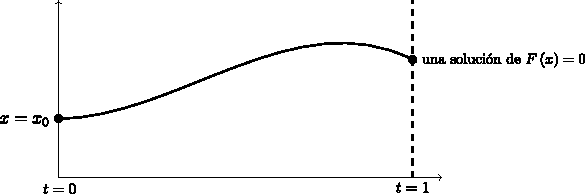
\includegraphics[width=0.65\paperwidth]{homotopy}
			\caption{
				Una curva suave definida por $H\left(x,t\right)=0$ alcanzando
				una solución $x^{\ast}$ del sistema objetivo.
			}
		\end{figure}
	\end{alertblock}

	\begin{definition}[Homotopía de punto fijo]
		Sean
		\begin{math}
			F\colon\mathbb{R}^{n}\times\mathbb{R}^{n}
		\end{math}
		y
		\begin{math}
			x=\left(x_{1},\dotsc,x_{n}\right)\in\mathbb{R}^{n}
		\end{math}.
		Una de las homotopías más sencillas para encontrar soluciones de
		$F\left(x\right)=0$ es la \alert{homotopía de punto fijo} dada
		por
		\begin{equation*}
			H\left(x,t\right)\coloneqq
			\left(1-t\right)\left(x-a\right)+tF\left(x\right),
		\end{equation*}
		donde $a\in\mathbb{R}^{n}$ y
		$t\in\left[0,1\right]\subset\mathbb{R}$.
		En $t=0$, el sistema inicial es $H\left(x,0\right)=x-a$
		para el cual la única solución es $x=a$.
		En $t=1$, el sistema $H\left(x,1\right)=F\left(x\right)=0$ es el
		sistema de interés.
	\end{definition}
	La suavidad de esta construcción de homotopía está garantizada por
	el teorema de Sard.
	\begin{theorem}[Teorema de Sard]
		Sean $X\subset\mathbb{R}^{n_{1}}$ e $Y\subset\mathbb{R}^{n_{2}}$
		dos conjuntos abiertos, $\phi\colon X\times Y\to\mathbb{R}^{m}$
		suave.
		Si $v\in\mathbb{R}^{m}$ es un punto regular de $\phi$, entonces
		para casi todo $y\in Y$, $v$ es un punto regular de
		$\pi_{Y}\colon X\to\mathbb{R}^{m}$.
	\end{theorem}

	\begin{definition}[Valor regular]
		Sea $F\colon\mathbb{R}^{n}\to\mathbb{R}^{p}$ suave.
		Un punto $y\in\mathbb{R}^{p}$ es \alert{valor regular} de $F$ sii
		\begin{equation*}
			\forall x\in F^{-1}\left(\left\{y\right\}\right)\coloneqq
			\left\{
			x\in\mathbb{R}^{n}\mid
			F\left(x\right)=y
			\right\}:
			\operatorname{rango}\left(DF\left(x\right)\right)=p.
		\end{equation*}
	\end{definition}
\end{frame}

\begin{frame}
	\frametitle{Método explícito de Runge-Kutta}
	La derivación sistemática de los métodos de un paso de orden
	superior se remonta a Runge y Kutta, quienes desarrollaron métodos
	especiales de tercer y cuarto orden hace más de $122$ años.

	\begin{definition}[Runge-Kutta explícito de $m$ etapas]
		Un método se denomina \alert{Runge-Kutta explícito de $m$ etapas}
		sii la función del método $f_{h}$ es una combinación lineal de
		valores de la función $f\left(x,y\right)$ en diferentes puntos
		$\left(x,y\right)$ es
		\begin{math}
			f_{h}\left(x,y\right)=
			\gamma_{1}k_{1}\left(x,y\right)+
			\gamma_{2}k_{2}\left(x,y\right)+
			\cdots+
			\gamma_{m}k_{m}\left(x,y\right)
		\end{math}
		con
		\begin{columns}
			\begin{column}{0.48\textwidth}
				\begin{align*}
					k_{1}\left(x,y\right) & =
					f\left(
					x,y
					\right)                                 \\
					k_{2}\left(x,y\right) & =
					f\left(
					x+\alpha_{2}h,
					y+h\beta_{21}k_{1}\left(x,y\right)
					\right).                                \\
					k_{3}\left(x,y\right) & =
					f\left(
					x+\alpha_{3}h,
					y+h\left[\beta_{31}k_{1}\left(x,y\right)+\beta_{32}k_{2}\left(x,y\right)\right]
					\right)                                 \\
					                      & \vdotswithin{=} \\
					k_{m}\left(x,y\right) & =
					f\left(x+\alpha_{m}h,y+h\sum\limits_{j=1}^{m-1}\beta_{mj}k_{j}\left(x,y\right)\right),
				\end{align*}
			\end{column}
			\begin{column}{0.48\textwidth}
				\begin{equation*}
					\begin{array}
						{c|ccccc}
						0                                                                    \\
						\alpha_{2} & \beta_{21}                                              \\
						\alpha_{3} & \beta_{31} & \beta_{32}                                 \\
						\vdots     & \vdots     &            & \ddots                        \\
						\alpha_{m} & \beta_{m1} & \beta_{m2} &        & \beta_{mm-1}         \\
						\hline
						           & h_{1}      & h_{2}      & \cdots & h_{m-1}      & h_{m}
					\end{array}
				\end{equation*}
				Este método será \alert{consistente} sii
				\begin{math}
					\sum\limits_{j=1}^{m}
					h_{j}=1
				\end{math}.
			\end{column}
		\end{columns}
		donde $x=x_{j}$, $y=u_{j}$ y $h=h_{j}$ para el paso $j$.

		Por lo tanto, el método se determina fijando
		$2m-1+\dfrac{m\left(m-1\right)}{2}$ parámetros
		\begin{equation*}
			\left\{
			\gamma_{1},\dotsc,\gamma_{m},
			\alpha_{2},\alpha_{3},\dotsc,\alpha_{m},
			\beta_{21},\beta_{31},\beta_{41}\dotsc,\beta_{mm-1}
			\right\}\subset
			\mathbb{R}.
		\end{equation*}
	\end{definition}
\end{frame}

\begin{frame}
	El método clásico de Runge-Kutta es
	\begin{align*}
		k_{1}   & = f\left(x_{j},u_{j}\right).                                        \\
		k_{2}   & = f\left(x_{j}+\dfrac{h_{j}}{2},u_{j}+\dfrac{h_{j}}{2}k_{1}\right). \\
		k_{3}   & = f\left(x_{j}+\dfrac{h_{j}}{2},u_{j}+\dfrac{h_{j}}{2}k_{2}\right). \\
		k_{4}   & = f\left(x_{j}+h_{j},u_{j}+h_{j}k_{3}\right).                       \\
		u_{j+1} & = u_{j}+\frac{h_{j}}{6}\left(k_{1}+2k_{2}+2k_{3}+k_{4}\right).      \\
	\end{align*}
\end{frame}

\begin{frame}
	\begin{enumerate}\setcounter{enumi}{33}
		\item

		      Use el método de continuación y el método explícito de
		      Runge-Kutta de orden cuatro en el sistema no lineal
		      \begin{align*}
			      10x_{1}-2x^{2}_{2}-2x_{3}-5 & =0 \\
			      8x^2_{2}+4x^2_{3}-9         & =0 \\
			      8x_{2}x_{3}+4               & =0
		      \end{align*}
	\end{enumerate}

	\begin{solution}
		.
	\end{solution}
\end{frame}